%!TEX program=xelatex
\documentclass[12pt]{article}

\usepackage{ctex}
\usepackage{amsmath}
\usepackage{amssymb}
\usepackage{siunitx}
\usepackage{xfp}%c
\usepackage{pgfplots}
\usepackage{float}
\usepackage{graphicx} 
\usepackage{caption}
\usepackage{geometry}
\geometry{a4paper,left=2cm,right=2cm,top=2cm,bottom=2cm}

\usepackage{enumitem}

\tikzset{elegant/.style={smooth,thick,samples=50,magenta}}
% \usepackage{zhnumber}
% \renewcommand{\thesection}{\zhnum{section}}

\pagestyle{plain}
% empty 
% plain
% headings
% myheadings

\pagenumbering{arabic}
% arabic 1 2 3 4
% roman  i ii iii iv
% Roman  
% alph   a b c d
% Alph


\title{\fangsong《激光原理》\quad 第二章\; 开放腔高斯光 习题}
%\date{}
\author{2019112019物理学(基地班)童旭东}

\begin{document}
\maketitle

\subsection*{一、基本概念问题}

{\fangsong
1、回答激光器的基本知识:
\par \quad \quad 传统激光器的主要构成部件;
\par \quad \quad 光学谐振腔的主要分类;
\par \quad \quad 按照腔内傍轴光线几何偏折损耗的大小,开放式光学谐振腔的分类。
}

{\kaishu
\par 答:
\par 
传统激光器的主要构成部件:光学谐振腔、泵浦源、增益物质。
\par 
光学谐振腔的主要分类:
\par \quad \quad \quad \quad 
根据是否含有增益的工作物质将光学谐振腔分为有源腔和无源腔腔;
\par \quad \quad \quad \quad 根据是否封闭可以分为封闭腔和开放腔。
\par 
开放式光学谐振腔的分类:开放式光腔分为稳定腔、临界腔和非稳腔。
}
\\

{\fangsong
2、简述光学谐振腔的模式概念及其基本特征,并分析其与光子态的关系。
}

{\kaishu
\par 
光腔的模式:光学谐振腔内可能存在的电磁场的本征态
\par 
从光子的角度看:激光模式就是腔内可能区分的光子的状态
\par 
模的基本特征:
\par \quad\quad\quad\quad
(1)每一个模的电磁场分布
\par \quad\quad\quad\quad
(2)模的谐振频率
\par \quad\quad\quad\quad
(3)每一个模在腔内往返一次的损耗
\par \quad\quad\quad\quad
(4)与每一个模式相对应的激光束的发散角
}
\\

{\fangsong
3、开放式谐振腔的振荡模式符号表现形式及其各个符号字母的含义?
}
{\kaishu
\par 
开放式谐振腔的振荡模式符号表现形式(相长干涉):
\begin{align*}
    &\Delta \Phi
    =\frac{2\pi}{\lambda_q}\cdot 2L'
    =q\cdot 2\pi\\
    &\quad \frac{2\pi \nu_q}{c}\cdot 2L'=q\cdot 2\pi
\end{align*}
}
\\

{\fangsong
4、驻波腔的纵模规律及驻波腔额纵模间隔?
}
{\kaishu
\begin{align*}
    L'&=q\frac{\lambda_q}{2}\\
    \nu_q&=\frac{qc}{2L'}\\
    \Delta\nu_q&=\frac{c}{2L'}
\end{align*}
}

{\fangsong
5、考虑到腔镜的不完全反射损耗及腔内损耗,光学谐振腔的总损耗的表达式?
}
{\kaishu
\par  
不论损耗的起源如何,都可以引进“平均单程损耗因子”$\delta$来定量地加以描述。该因子的定义如下:如果初始光强为$I_0$,在无源腔内往返一次后,光强衰减$I_1$,则:
\begin{align*}
    &I_1=I_0e^{-2\delta}\\
    &\delta=\frac{1}{2}\ln\frac{I_0}{I_1}
    \quad\quad\quad
    \text{其中:}\delta=\sum_i \delta_i
\end{align*}
}

{\fangsong
6、无源腔的品质因数普遍定义及其含义,并推导其与腔内损耗的关系。
}
{\kaishu

设t时刻腔内光子数密度为N,
N与光腔I(t)的关系为:$I(t)=Nh\nu v$,相应的,初始时刻有:$I_0=N_0h\nu v $
\begin{align}
    &\text{光子在腔内的平均寿命关系:}
    I(t)
    =I_0(e^{-2\delta})^{\frac{t}{\frac{2L'}{c}}}
    =I_0e^{-\frac{t}{\tau_c}}\\
    &\text{进而可得:}N=N_0e^{-\frac{t}{\tau_R}}\\
    &\text{无源腔品质因数:}
    Q
    =\frac{\omega}{\Delta\omega_{\frac{1}{2}}}
    =\frac{\nu}{\Delta\nu_{\frac{1}{2}}}
    =\omega\frac{E}{P}
\end{align}
\par 式中,
$E=Nh\nu V$是存在腔内的总能量;
$P$为单位时间内损耗的能量;
$\nu$为腔内电磁场的振荡频率;
$\omega=2\pi\nu$为场的角频率。
\begin{align}
    &\text{单位时间中光能的减少(能量损耗):}
    P
    =-\frac{\mathrm{d}E}{\mathrm{d}t}
    =-h\nu V\frac{\mathrm{d}N}{\mathrm{d}t}\\
    &\text{品质因数:}Q
    =\omega\frac{E}{P}=
    \omega\left|
    \frac
    {Nh\nu V}
    {-h\nu V\frac{\mathrm{d}N}{\mathrm{d}t}}
    \right|
    =
    \left|\omega\frac{N}{\frac{\mathrm{d}N}{\mathrm{d}t}}\right|
    =\omega\tau_c
\end{align}
}

{\fangsong
7、复杂开腔的稳定性条件及共轴球面腔的稳定性条件?绘制共轴球面腔稳定性曲线,标出平行平面腔、共心腔、对称共焦腔、临界腔、稳定腔和非稳定腔的位置,并给出其满足的条件。
}

{\kaishu
复杂开腔的稳定性条件:

\begin{figure}[H]
\begin{center}
\begin{tikzpicture}[scale=1, transform shape]
    % the axis environment 
    \begin{axis}[axis x line=middle,
                 axis y line=middle,
                 ylabel=$g_1$,
                 xlabel=$g_2$]
        \addplot[elegant,orange,domain=-pi:-1/pi]{1/x};
        \addplot[elegant,orange,domain=1/pi:pi]{1/x};	
	\end{axis}
\end{tikzpicture}
\end{center}
\caption*{图1.1}%
\end{figure}
\par 稳定腔:$ 0 < g_1g_2 < 1$,在双曲线之间;
\par 临界腔:$  g_1g_2 = 1$或$g_1g_2=0$,在双曲线上;
\par 非稳腔:$g_1g_2<0$ 或 $g_1g_2>1$ ,在双曲线外
\\


}

{\fangsong
8、开腔中自再现模满足的本征方程及其各物理量的含义。
}
{\kaishu
\begin{equation*}
	v(x,y)=\frac{i\gamma}{L\lambda} \iint_{{S'}}^{{}} {v(x',y')e^{-ikr}} \: d{S'} {}
\end{equation*}
$v(x,y)$式在镜面 $S$ 和$S'$ 的场分布, $r=\sqrt{(x-x')^2+(y-y')^2+(z-z')^2}$,$\gamma$ 为渡跃系数,为一个常数
\\}

{\fangsong
9、方形/圆形球面镜对称共焦腔腔镜面上的自再现模遵从的精确解,近似解的表达形式及各物理量含义,腔内、腔外行波场的表达形式。
}
{\kaishu
\par 方形镜自在现模:
\begin{equation*}
	v_{mn}(x,y)
	=
	S_{om}\left(c,\frac{x}{a} \right)
	S_{on}\left( c,\frac{y}{a} \right)
	=C_{mn}
	H_m \left( \sqrt{\frac{2\pi}{L\lambda} }x \right)
	H_n \left( \sqrt{\frac{2\pi}{L\lambda} } y\right)
	e^{-\frac{x^2+y^2}{L\lambda/\pi} }
\end{equation*}
式中,$H(x)$ 是Hermit多项式
\par 方形行波场:
\begin{equation*}
	E_{mn}(x,y,z)=A_{mn}E_0 \frac{\omega_0}{\omega(z)} 
	H_m \left[ \frac{\sqrt2}{\omega(z)} x \right]
	H_n \left[ \frac{\sqrt2}{\omega(z)} y \right]
	e^{-\frac{r^2}{\omega^2(z)} }
	e^{-i\Phi(x,y,z)}
\end{equation*}
\par 圆形镜自在现模:
\begin{equation*}
	v_{mn}(r,\varphi)
	=C_{mn}\left( \sqrt{2}\frac{r}{\omega_{0_s}}  \right)
	 L_n^m \left( 2 \frac{r^2}{\omega_{0_s}^2}  \right)
	 e^{-\frac{r^2}{\omega_{0s}^2} } 
	\begin{cases}
		\cos m\phi &\\
		\sin m\phi
	\end{cases}
\end{equation*}
\par 圆形行波场:
\begin{equation*}
	E_{mn}(r,\varphi,z)=A_{mn}E_0 \frac{\omega_0}{\omega(z)} 
	\left[ \sqrt2 \frac{r}{\omega(z)}  \right]^m
	L_n^m \left[ 2 \frac{r^2}{\omega^2(z)}  \right]
	e^{-\frac{r^2}{\omega^2(z)}} e^{-im\varphi} e^{-i\Phi(x,y,z)}
\end{equation*}
\\}

{\fangsong
10、方形/圆形球面镜对称共焦腔腔镜面上中任何位置z处的基模光斑半径表达式。
}
\begin{equation*}
	\omega(z)=
	\sqrt{\frac{L\lambda}{2\pi} \left( 1+ \frac{z^2}{f^2}  \right)} 
	= \omega_{0_s}\sqrt{1+\frac{z^2}{f^2} }
\end{equation*}

{\fangsong
11、方形/圆形球面镜对称共焦腔行波场的等相位面分布是如何随着位置z发生变化的,试绘图进行说明。
}

{\fangsong
12、共焦腔模式理论可以推广到一般两镜稳定球面腔,试证明之。
}

{\fangsong
13、基膜高斯光束的场分布函数,光斑半径、等相位面曲率、共焦参数、远场发散角、q参数及其变化规律,聚焦、准直和放大。
}
{\kaishu \noindent
\par 基膜高斯光束分布函数:
\[
	\psi_{00}\left( x,y,z \right) =\frac{c}{\omega(z)} 
	e^{-\frac{r^2}{\omega^2(z)} }
	e^{-i \left[ k \left( z+\frac{r^2}{2R}  \right) -\arctan \frac{z}{f}  \right] }
\]
\par 光斑半径:
\[
	\omega(z) = \omega_0 \sqrt[]{1+\left( 1+\frac{z}{f}  \right) ^2 } 
		 =\omega_0 \sqrt[]{1+\left( \frac{\lambda z}{\pi \omega_0^2}  \right) ^2}  
\]
\par 等相位面曲率半径:
\[
	R(z)=z \left[ 1+\left( \frac{f}{z}  \right) ^2 \right] = f \left( \frac{z}{f} +\frac{f}{z}  \right) 
\]
\par 共焦参数:
\[
	f=\frac{\pi\omega_0^2}{\lambda} 
\]
\par 在基模高斯光束强度的$\dfrac{1}{e} $处远场发散角为:
\[
	\theta_0 = \lim_{z \to \infty} \frac{2\omega(z)}{z} = 2 \frac{\lambda}{\pi\omega_0} =2 \sqrt[]{\frac{\lambda}{\pi f} } 
\]
\par q参数:
\[
	 \frac{1}{q(z)} = \frac{1}{R(z)} - i \frac{\lambda}{\pi\omega^2(z)} 
\]
\par q参数ABCD公式:
\[
	q_2 = \frac{Aq_1+B}{Cq_1+D} 
\]
\par 聚焦:
\[
	\begin{cases}
		\omega_0'\approx \dfrac{\lambda}{\pi\omega_0} F,l'=F &\text{F一定,$\omega_0'$随l变化的情况}\\
		\omega_0'=\dfrac{\lambda}{\pi\omega_0} F &\text{$l>F$}\\
		\omega_0' = \frac{\lambda}{\pi\omega_0} F &\text{$l'=F$}
	\end{cases}
\]
\par 准直:
\[
	M'= \frac{\theta_0"}{\theta_0} 
\]
\\}

{\fangsong
14、高斯光束的自再现变换规律(证明)
}
\newpage



\subsection*{二、计算题}
1、Consider a F-P interferometer made of a piece of glass with two
plane-parallel surfaces coated for high reflectivity. If we asumme L=1cm
and $n_r$=1.54, the free-spectral range for near normal incidence will be? If
we take R1=R2=0.98, the interferometer finesse and the resolution
(linewidth of the transmission peak) will be?
\par 解:
	\begin{align*}
		&\Delta\nu_{FSR}=\frac{c}{2n_r L} = \frac{3\times10^8}{2\times1.54\times0.01} = 9.7\times10^9 \si{Hz}
	  \\& \Delta\nu_{\frac{1}{2} }=\frac{c}{2\pi n_r L} \frac{1-(r_1r_2)^{\frac{1}{2} }}{(r_1r_2)^{\frac{1}{4} }} =6.3\times 10^7 \si{Hz}
	  \\& F=\frac{\Delta_{FSR}}{\Delta\nu_{\frac{1}{2} }} =154
	\end{align*}

{\fangsong
2. 试利用往返矩阵证明共焦腔为稳定腔,即任意傍轴光线在其中可以往
返无限多次,而且两次往返即自行闭合。
}
\begin{figure}[H]
	\centering
	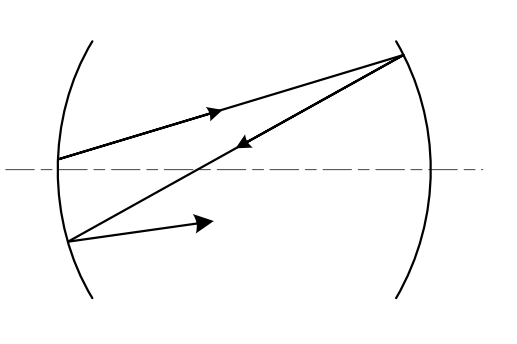
\includegraphics[width=0.3\linewidth]{fig/1_new.png}
	\caption*{}%
\end{figure}
{\kaishu\noindent
 解:
 \par 稳定腔条件:
 \begin{equation*}
 	\left| \dfrac{A+D}{2}  \right|<1
 \end{equation*}
\par 对于共焦腔,有:$R_1=R_2=L$
\par 对于一次往返,有:
 \begin{align*}
	 T&=
%\begin{bmatrix}
%	A & B \\
%	C & D 
%\end{bmatrix}
%=
\begin{bmatrix}
	1-\dfrac{2L}{R_2} & 2L \left( 1- \dfrac{L}{R_2}  \right)\\
	-\left[\dfrac{2}{R_1} + \dfrac{2}{R_2} \left( 1-\dfrac{2L}{R_1}  \right)\right]
	& 
	-\left[ \dfrac{2L}{R_1} -\left( 1-\dfrac{2L}{R_1}  \right)\left( 1-\dfrac{2L}{R_2}  \right) \right]
\end{bmatrix}
\\&=
\begin{bmatrix}
	1-\dfrac{2L}{L} & 2L \left( 1- \dfrac{L}{L}  \right)\\
	-\left[\dfrac{2}{L} + \dfrac{2}{L} \left( 1-\dfrac{2L}{L}  \right)\right]
	& 
	-\left[ \dfrac{2L}{L} -\left( 1-\dfrac{2L}{L}  \right)\left( 1-\dfrac{2L}{L}  \right) \right]
\end{bmatrix}
\\&=
\begin{bmatrix}
	-1 & 0 \\
	0 & -1
\end{bmatrix}
\\
 \end{align*}

\newpage 
\par 显然,共焦腔符合稳定腔条件 $\left( \left| \dfrac{A+D}{2}  \right|=0<1 \right)$
\par 两次往返:
\begin{equation*}
	\begin{bmatrix}
		r_1 \\ \theta_1
	\end{bmatrix}
	T^2=
	\begin{bmatrix}
		r_0 \\ \theta_0
	\end{bmatrix}
	\begin{bmatrix}
		1 & 0 \\
		0 & 1
	\end{bmatrix}
	=
	\begin{bmatrix}
		r_0 \\ \theta_0
	\end{bmatrix}
\end{equation*}
\\}

{\fangsong
3. 激光器的谐振腔由一面曲率半径为 1m 的凸面镜和曲率半径为 2m 的
凹面镜组成,工作物质长 0.5m,其折射率为 1.52,求腔长 L 在什么
范围内是稳定腔。
}
{\kaishu\noindent
\\解:
\par 设腔的光学长度为$L'=L+0.5 \times 0.52$
\par 据题意,$R_1=-1,R_2=2$
\[
	\frac{A+D}{2} 
	=1-\frac{2L'}{R_1} -\frac{2L'}{R_2} +\frac{2L'^2}{R_1R_2} 
	=1+L'-L'^2
	=-(L'-\frac{1}{4})^2+\frac{5}{4}  
	=-(L-0.1)^2+\frac{5}{4}  
\]
\par 解得:
\[
	L>0.1+\frac{\sqrt[]{7}}{2}\quad or\quad L<-0.1-\frac{\sqrt[]{7}}{2} 
\]
\\}

{\fangsong
4.图 2.1 所示三镜环形腔,已知$l$,试画出其等效透镜序列图,并求球面
镜的曲率半径 R 在什么范围内该腔是稳定腔。图示环形腔为非共轴球面
镜腔。在这种情况下,对于在由光轴组成的平面内传输的子午光线,式
(2.2.7)中的 $f=(R\cos\theta)/{2}$,对于在与此垂直的平面内传输的弧矢光线,
$f=R/(2\cos\theta)$,$\theta$为光轴与球面镜法线的夹角。
}
\begin{figure}[H]
	\centering
	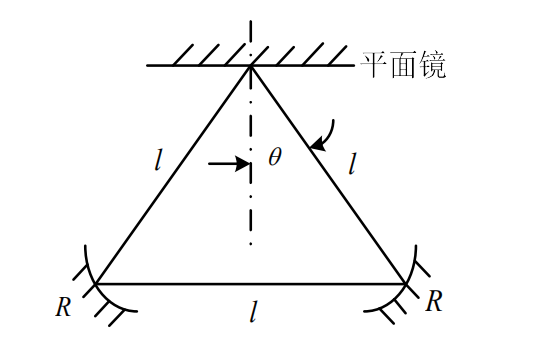
\includegraphics[width=0.5\linewidth]{fig/4_new.png}
	\caption*{图2.1}%
\end{figure}
{\kaishu\noindent
\\解:
\par 由平面镜右侧光束起,先后经过平面镜反射、自由传播、左侧球面镜反射、自由传播、右侧球面镜反射、自由传播几个过程,即:
\[
	T=T_{\infty}T_FT_RT_FT_RT_F
\]
\par 其中,$T_{\infty}=E$,则,传输矩阵为:
\begin{align*}
	T=&
	E
	\begin{bmatrix}
		1 & L \\
		0 & 1
	\end{bmatrix}
	\begin{bmatrix}
		1 & 0 \\
		-\dfrac{1}{f}  & 1
	\end{bmatrix}
	\begin{bmatrix}
		1 & L \\
		0 & 1
	\end{bmatrix}
	\begin{bmatrix}
		1 & 0 \\
		-\dfrac{1}{f}  & 1
	\end{bmatrix}
	\begin{bmatrix}
		1 & L \\
		0 & 1
	\end{bmatrix}
	\\=&
	\begin{bmatrix}
		\left(  1-\dfrac{L}{f}\right)^2 -\dfrac{L}{f} & L \left[ \left( 1-\dfrac{L}{f}  \right)^2-\dfrac{L}{f}   \right] + \left[ \left( 1-f \right) L-\dfrac{1}{f}  \right] \\
		\left( 1-\dfrac{L}{f}  \right)  \left( -\dfrac{1}{f}  \right)+L & L \left[  	\left( 1-\dfrac{L}{f}  \right)  \left( -\dfrac{1}{f}  \right) \right] -\dfrac{L}{f} + 1
	\end{bmatrix}
\end{align*}
\[
	\dfrac{A+D}{2} = \left( 1-\dfrac{L}{f}  \right) ^2-\dfrac{L}{f} 
\]
\[
	1 > \left( \dfrac{L}{f}  \right) ^2 -3 \dfrac{L}{f} +1 > -1	
\]
\par 解得:
\[
	\frac{L}{f} \in \{ x|x<0,x>3\text{且}2>x>1 \}
\]
\[
	f\in \left( \frac{L}{3} ,\frac{L}{2}  \right) \cup	\left( L,+\infty \right) 
\]
\\}

{\fangsong
5. 有一方形孔径的共焦腔氦氖激光器,$L=30\si{\cm}$,$d=2a=0.12\si{\cm}$,
$\lambda=632.8\si{\nm}$ ,镜的反射率为$r_1=1,r_2=0.96$,其他的损耗以每程 0.003 估计。
此激光器能否作单模运转?如果想在共焦镜面附近加一个方形小孔
阑来选择$\mathrm{TEM_{00}}$ 模,小孔的边长应为多大?试根据图 2.5.5 作一个大略
的估计。\\氦氖增益由公式计算。$ e^{g^{0_l}}=1+3\times10^{-4}\dfrac{l}{d} $
}
{\kaishu\noindent
\\解:
%\par 衍射损耗的大小:$\delta_{00}=10.9\times10^{-4.94N}$
%\par 单程损耗:
%\[
%	\delta=\delta_r+
%\]
\[
	\omega_{0_s}=\sqrt[]{\dfrac{L\lambda}{\pi} }=2.46\times10^{-2}\si{cm}
\]
\\}

{\fangsong
6.试分别用解析解法和数值迭代方法计算方形球面镜/圆形镜对称共焦腔
镜面上基模、$\mathrm{TEM_{10}}$、$\mathrm{TEM_{20}}$、$\mathrm{TEM_{21}}$
模式的场分布情况,并分别比较其误差。
}
{\kaishu\noindent
\par 方形球面镜:
\begin{align*}
	  &\mathrm{TEM_{00}}=C_{00}e^{-\frac{X^2+Y^2}{\omega^2_{0_s}} }
	\\&\mathrm{TEM_{10}}=C_{10} 2X e^{-\frac{X^2+Y^2}{\omega^2_{0_s}} }
	\\&\mathrm{TEM_{20}}=C_{20} \left( 4X^2-2 \right) e^{-\frac{X^2+Y^2}{\omega^2_{0_s}} } 
	\\&\mathrm{TEM_{21}}=C_{20} \left( 4X^2-2 \right)2Y e^{-\frac{X^2+Y^2}{\omega^2_{0_s}} } 
\end{align*}
\par 圆形球面镜:
\begin{align*}
	&\mathrm{TEM_{00}}=C_{00}e^{-\frac{r^2}{\omega^2_{0_s}} }
  \\&\mathrm{TEM_{10}}=C'_{10}re^{-\frac{r^2}{\omega^2_{0_s}} }
  \begin{cases}
	  \cos\varphi\\\sin\varphi
  \end{cases}
  \\&\mathrm{TEM_{20}}=C'_{20}r^2e^{-\frac{r^2}{\omega^2_{0_s}} }
  \begin{cases}
	  \cos2\varphi\\\sin2\varphi
  \end{cases}
  \\&\mathrm{TEM_{21}}=C'_{21}r^2 \left( 3-\frac{2r^2}{\omega^2_{0_s}}  \right)  e^{-\frac{r^2}{\omega^2_{0_s}} }
  \begin{cases}
	  \cos2\varphi\\\sin2\varphi
  \end{cases}
\end{align*}
\\}

{\fangsong
7.试求出方形镜共焦腔面上$\mathrm{TEM_{30}}$模的节线位置,这些节线是等距分布
的吗?
}
{\kaishu\noindent
\\解:
\par 方形球面镜,傍轴条件,可用Hermit-Gauss函数表示镜面上场的函数
\[
	\nu_{30}=C_{30}
	H_3 \left( \sqrt[]{\dfrac{2\pi}{L\lambda} }x \right) 
	H_0 \left( \sqrt[]{\dfrac{2\pi}{L\lambda} }y \right) 
	e^{-\frac{x^2+y^2}{L\lambda/\pi} }=0
\]
\[
	8X^3-12X=0
\]
\[
	X_1=0,X_2=-\sqrt[]{\frac{3}{2} },X_3=\sqrt[]{\frac{3}{2} }
\]
\par 是等距的
\\}

{\fangsong
8.试通过公式(2.8.6)积分计算腔长为 L 的激光器的模体积,并与公式
(2.8.8)对比体积误差。
}
{\kaishu\noindent
\par 由$\omega(z)=\omega_{0_s}\sqrt[]{1+\dfrac{z^2}{f^2} }$
\begin{align*}
	V&
=\int_{{z_1}}^{{z_2}} {\pi\omega^2(z)} \: \mathrm{d}{z} {}
=\int_{{z_1}}^{{z_2}} {\pi\omega_{0_s}^2 \left( 1+\dfrac{z^2}{f^2}  \right)  } \: \mathrm{d}{z} {}
	=\pi\omega_{0_s}^2 \left[ (z_2-z_1)+\dfrac{z_2^3-z_1^3}{3f^2}  \right] 
\end{align*}
\par 直接计算: 
\[
	V'=\frac{1}{2} \pi L \left( \frac{\omega_{s_1}+\omega_{s_2}}{2}  \right) ^2
\]
\\}

{\fangsong
9.今有一球面腔,$R_1=1.5\si{\m}$,$R_2=-1\si{\m}$,$L=80\si{\cm}$。
试证明该腔为稳定腔;
求出它的等价共焦腔的参数;在图上画出等价共焦腔的具体位置。
}
{\kaishu\noindent
\\证明:
\[
 g_1g_2
 =\left(1-\frac{L}{R_1} \right)\left( 1-\frac{L}{R_2}  \right) 
 =\left( 1-\frac{8}{15}  \right) \left( 1+\frac{8}{10}  \right) 
 =\frac{21}{25} <1
\]
\par 稳定腔得证
\begin{align*}
	&z_1=\frac{L(R_2-L)}{(L-R_1)+(L-R_2)} = \frac{0.8(-1-0.8)}{2\times0.8+1.5-1} = \fpeval{-0.8*1.8/2.1}
\\	&z_2=\frac{-L(R_1-L)}{(L-R_1)+(L-R_2)} = \frac{0.8(1.5-0.8)}{2\times0.8+0.5} = \fpeval{0.8*0.7/2.1}
\\	&f^2=\frac{L(R_1-L)(R_2-L)(R_1+R_2-R)}{[(L-R_1)+(L-R_2)]^2} 
=\fpeval{0.8*(-1-0.8)*(1.5-0.8)*(-0.3)/2.1^2}
\end{align*}
\\}

{\fangsong
10.方形镜对称共焦腔焦参数$f=0.4\si{m}$,光波长$\lambda=0.314\si{\um}$,
求腰斑半径、镜面处光斑半径与等相位面曲率半径。
}
{\kaishu\noindent
解:
\begin{align*}
	&\omega_0=\sqrt[]{\frac{L\lambda}{2\pi} }=\sqrt[]{\frac{f\lambda}{\pi} }=\fpeval{0.4*0.314/3.14}\si{\um}
	\\&\omega_{0_s}=\sqrt[]{2}\omega_0=\fpeval{sqrt(2)*0.04}\si{\um}
	\\&R=z+\frac{f^2}{z} =2f=0.8\si{m}
\end{align*}
\\}

{\fangsong
11.某高斯光束腰斑半径大小为$\omega_0=1.14\si{\mm}$,$\lambda=10.6\si{\um}$。
求与束腰相距30cm、10m、1000m远处的光斑半径$\omega$及波前曲率半径R。
}
{\kaishu\noindent
\par 远处光斑半径:$\omega=\omega_0 \sqrt[]{1+\dfrac{z^2}{f^2} }$,
波前曲率半径:$R=z+\dfrac{f^2}{z} $
\par 由腰斑半径关系$\omega_0=\sqrt[]{\dfrac{L\lambda}{2\pi} }=\sqrt[]{\dfrac{f\lambda}{\pi} }$ ,$f=\dfrac{\pi\omega_0^2}{\lambda}=\fpeval{3.14*1.14*1.14/10.6}\si{m} $
\par 30cm: 
\[
	\omega=1.14\times \sqrt[]{1+\frac{0.3\times0.3}{0.385\times0.385} }	
\]
\\}

{\fangsong
12.(a)计算腔长为1m的共焦腔基横模的远场发散角,设
$\lambda=6328$ $\mathring{\mathrm{A}}$
,10km处的光斑面积多大。
(b)有一普通探照灯,设发散角为$2^\circ$,则1km远
处的光斑面积多大?
}
{\kaishu\noindent
	\par (a) $\theta=\dfrac{\omega(z)}{z} 
	=\dfrac{\sqrt[]{\frac{l\lambda}{2\pi} }\sqrt[]{1+\frac{z^2}{f^2} }}{z} 
	=2 \sqrt[]{\dfrac{\lambda}{\pi f} }$
	\par $\omega=\omega_0 \sqrt[]{1+\frac{z^2}{f^2} }$
	\par (b)$(l\theta)^2\pi$
\\}

{\fangsong
	14. 已知波长$\lambda=0.6328\si{\um}$的两高斯光束的束腰半径$\omega_{10}$、$\omega_{20}$
	分别为$0.2\si{\mm}$、$50\si{\um}$,试问此二光束的远场发散角分别为多少?后者是前者的几倍?
}
{\kaishu\noindent
\par $\theta=2 \sqrt[]{\dfrac{\lambda}{\pi f} }=\frac{2\lambda}{\pi\omega_0} $
\\}

{\fangsong
15.激光的远场发散角$\theta$ (半角)还受到衍射效应的限制。它不能小于激光
通过输出孔时的衍射极限角$ \theta_{\text{衍}}$ (半角)=1.22$\lambda$/d。在实际应用中远场发
散角常用爱里斑衍射极限角来近似。试计算腔长为 30cm 的氦氖激光
器,所发波长$\lambda$=6328Å的远场发散角和以放电管直径 d=2mm 为输
出孔的衍射极限角。
}
{\kaishu\noindent
	$$\theta=2 \sqrt[]{\dfrac{\lambda}{\pi f} }$$
\\}

{\fangsong
	16.一共焦腔(对称)$L=0.40\si{m}$,$\lambda=0.6328\si{\um}$,
	束腰半径$\omega_0=0.2\si{\mm}$,求离腰56cm处的光束有效截面半径。
}
{\kaishu\noindent
	\[
		\omega=\omega_0 \sqrt[]{1+\dfrac{z^2}{f^2} }
	\]
\\}

{\fangsong
17. 试讨论非共焦腔谐振频率的简并性、纵模间隔及横模间隔,并与共焦
腔进行比较。
}
{\kaishu\noindent
	mn简并
\\}

{\fangsong
18. 考虑一用于氩离子激光器的稳定球面腔,波长$\lambda=0.5145\si{\um}$,腔长 L
=1m,腔镜曲率半径 $R_1=1.5$m,$R_2=4$m。试计算光腰尺寸和位置,两
镜面上的光斑尺寸,并画出等效共焦腔的位置。
}
{\kaishu\noindent
\begin{align*}
	&z_1=\frac{L(R_2-L)}{(L-R_1)+(L-R_2)} 
\\	&z_2=\frac{-L(R_1-L)}{(L-R_1)+(L-R_2)} 
\\	&f^2=\frac{L(R_1-L)(R_2-L)(R_1+R_2-R)}{[(L-R_1)+(L-R_2)]^2} 
\end{align*}
\\}

{\fangsong
19. 欲设计一对称光学谐振腔,波长$\lambda=10.6\si{\um}$,两反射镜间距 L=2m,
如选择凹面镜曲率半径 R=L,试求镜面上光斑尺寸。若保持 L 不变,
选择 $R \gg L$,并使镜面上的光斑尺寸$w_s$=0.3cm,问此时镜的曲率半
径和腔中心光斑尺寸多大?
}
{\kaishu\noindent
	\par (1)$R=L$,对称共焦腔
	\[
		\omega_{0_s}=\sqrt[]{\dfrac{L\lambda}{\pi} }=2.6\si{\mm}
	\]
	\par (2)
	\[
		\omega_s=\omega_{0_s}\left[ \dfrac{g_1}{g_1(1-g_1g_2}  \right] ^{\frac{1}{4} }
	\]
	\[
	f^2=\frac{L(R_1-L)(R_2-L)(R_1+R_2-R)}{[(L-R_1)+(L-R_2)]^2} 
	\]
	\[
		\omega=\sqrt[]{\dfrac{f\lambda}{\pi} }
	\]
\\}

{\fangsong
	20. 若已知某高斯光束之$\omega_0=0.3$mm,$\lambda=632.8\si{\nm}$。求束腰处的q参数值,
与束腰相距 30cm 处的q参数值,以及在与束腰相距无限远处的q值。
}
{\kaishu\noindent
	\[
		q_2=q_1+(z_2-z_1)=q_1+L
	\]
	\par $z=0$束腰:$q_{z=0}=-i \dfrac{\pi\omega^2}{\lambda} $
	\par $z=30$束腰: $q_{z=30}=q_{z=0}+(30-0)$
\\}


{\fangsong
	21. 某高斯光束$\omega_0=1.2$mm,$\lambda=10.6\si{\um}$。今用 F=2cm 的锗透镜来聚焦,当
束腰与透镜的距离为 10m、1m、10cm、0 时,求焦斑的大小和位置,
并分析所得的结果。
}
{\kaishu\noindent
	\par 由$\omega_0'^2=\dfrac{F^2\omega_0^2}{(F-l)^2+\left( \dfrac{\pi\omega_0^2}{\lambda}  \right) ^2} $
\\}

{\fangsong
22. 一高斯光束束腰半径$\omega_0=0.2\si{mm}$,$\lambda=0.6328\si{\um}$,
今用一焦距 f 为 3cm的短焦距透镜聚焦,已知腰粗$\omega_0$离透镜的距离为 60cm,在几何光学
近似下求聚焦后光束腰粗。
}

{\fangsong
	23. CO$_2$激光器输出光$\lambda=10.6\si{\um}$,$\omega_0=3\si{mm}$,
	用一 F=2cm 的凸透镜距角,求
	欲得到$\omega=20\si{\um}$及$2.5\si{\um}$时透镜应放在什么位置。
}


{\fangsong
	24.入射光$\lambda=10.6\si{\um}$,求$\omega_0^{''}\text{及}l_3$。
}

\begin{figure}[H]
	\centering
	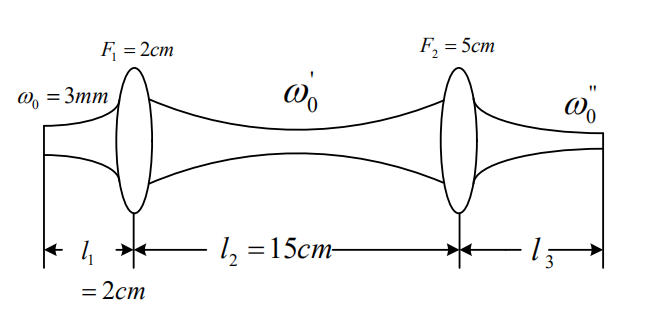
\includegraphics[width=0.6\linewidth]{fig/23_new.png}
	\caption*{图2.2}%
\end{figure}

{\fangsong
25. 某高斯光束$\omega_0=1.2$mm,$\lambda=10.6\si{\um}$。今用一望远镜将其准直。主镜用
镀金反射镜 R=1m,口径为 20cm;副镜为一锗透镜,$F_1$=2.5cm,口径
为 1.5cm;高斯束腰与透镜相距l=1m,如图 2.3 所示。求该望远系统
对高斯光束的准直倍率。
}
\begin{figure}[H]
	\centering
	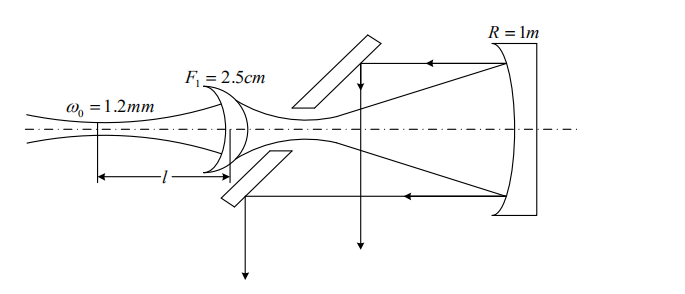
\includegraphics[width=0.6\linewidth]{fig/25_new.png}
	\caption*{图2.3}%
\end{figure}

{\fangsong
26.用如图(4 -33)所示的倒置望远镜系统改善由对称共焦腔输出的光
束方向性。已知二透镜的焦距分别为 $f_1$=2.5cm,$f_2$=20cm,$\omega_0$= 0.28mm,
$l_1\gg f_1$($L_1$紧靠腔的输出镜面),求该望远镜系统光束发散
角的压缩比。
}
\begin{figure}[H]
	\centering
	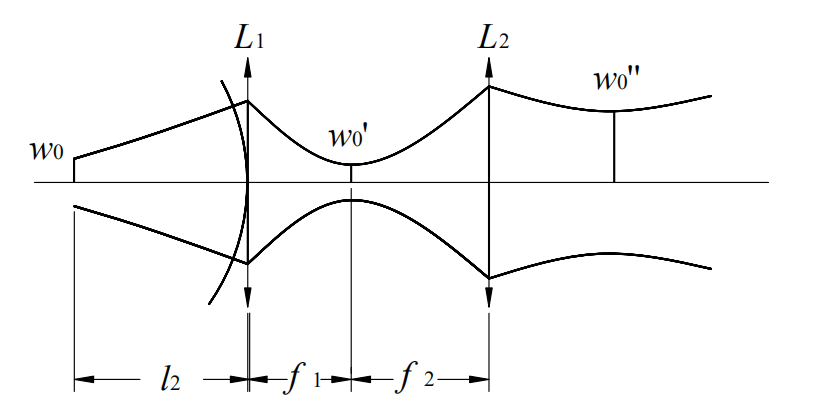
\includegraphics[width=0.6\linewidth]{fig/26_new.png}
	\caption*{图(4-33)}%
\end{figure}

{\fangsong
27.激光器的谐振腔有两个相同的凹面镜组成,它出射波长为$\lambda$ 的基模高
斯光束,今给定功率计,卷尺以及半径为 a 的小孔光阑,试叙述测量
该高斯光束公焦参数$f$的实验原理及步骤。
}


\end{document}


